% tikzpic.teP
\documentclass[crop,tikz]{standalone}% 'crop' is the default for v1.0, before it was 'preview'

%tikz libraries
\usetikzlibrary{shapes.geometric}

% Formatting macros:
\tikzstyle{node}=[circle, draw]
\tikzstyle{edge}=[diamond, draw]
\tikzstyle{intervention}=[fill = blue ,fill opacity= .3 ]
\tikzstyle{epidemic}=[fill = red,fill opacity= .3 ]
\tikzstyle{contact}=[fill opacity= .3 ]
\tikzstyle{initial}=[fill = green,fill opacity= .3 ]
\tikzstyle{inherits}=[-{LateP[length=5mm, width=2mm]},dashed]
\tikzstyle{member}=[-{LateP[length=5mm, width=2mm]},blue]


\begin{document}

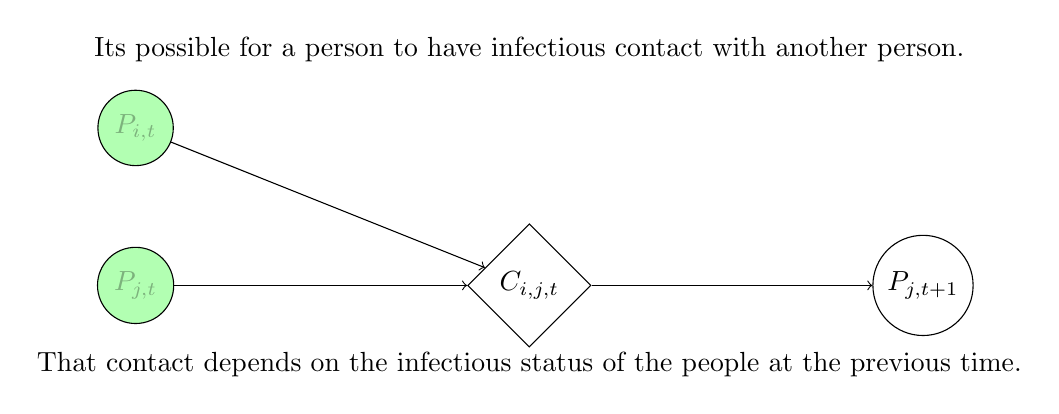
\begin{tikzpicture}
\draw (5,3) node {Its possible for a person to have infectious contact with another person.};
\draw (0,2) node[initial, node] (P11) {$P_{i,t}$};
\draw (0,0) node[initial, node] (P21) {$P_{j,t}$};
\draw (10,0) node[node] (P22) {$P_{j,t+1}$};
\draw (5,0) node[edge] (C121) {$C_{i,j,t}$};

\draw[->] (P11) -- (C121);
\draw[->] (P21) -- (C121);
\draw[->] (C121) -- (P22);
\draw (5,-1) node{That contact depends on the infectious status of the people at the previous time.};
\end{tikzpicture}

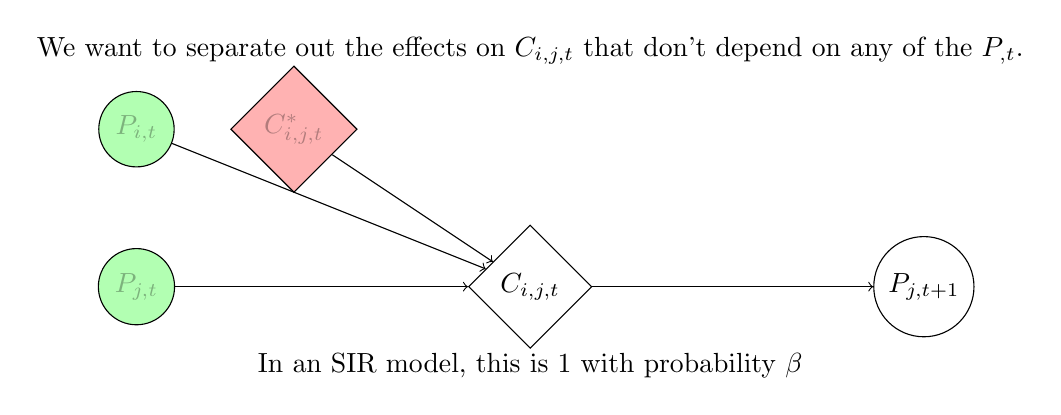
\begin{tikzpicture}
\draw (5,3) node {We want to separate out the effects on $C_{i,j,t}$ that don't depend on any of the $P_{,t}$.};
\draw (0,2) node[initial, node] (P11) {$P_{i,t}$};
\draw (0,0) node[initial, node] (P21) {$P_{j,t}$};
\draw (2,2) node[epidemic, edge] (E121) {$C^*_{i,j,t}$};
\draw (10,0) node[node] (P22) {$P_{j,t+1}$};
\draw (5,0) node[edge] (C121) {$C_{i,j,t}$};

\draw[->] (P11) -- (C121);
\draw[->] (P21) -- (C121);
\draw[->] (C121) -- (P22);
\draw[->] (E121) -- (C121);
\draw (5,-1) node{In an SIR model, this is $1$ with probability $\beta$};
\end{tikzpicture}

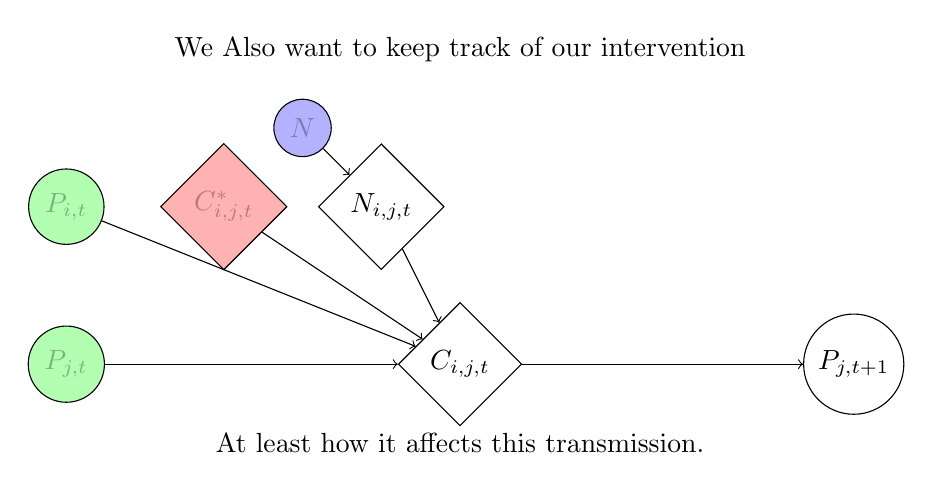
\begin{tikzpicture}
\draw (5,4) node {We Also want to keep track of our intervention};
\draw (0,2) node[initial, node] (P11) {$P_{i,t}$};
\draw (0,0) node[initial, node] (P21) {$P_{j,t}$};
\draw (2,2) node[epidemic, edge] (E121) {$C^*_{i,j,t}$};
\draw (3,3) node[intervention, node] (I) {$N$};
\draw (4,2) node[ edge] (I121) {$N_{i,j,t}$};
\draw (10,0) node[node] (P22) {$P_{j,t+1}$};
\draw (5,0) node[edge] (C121) {$C_{i,j,t}$};

\draw[->] (P11) -- (C121);
\draw[->] (P21) -- (C121);
\draw[->] (C121) -- (P22);
\draw[->] (E121) -- (C121);
\draw[->] (I121) -- (C121);
\draw[->] (I) -- (I121);
\draw (5,-1) node {At least how it affects this transmission.};
\end{tikzpicture}

\begin{tikzpicture}
\draw (5,4) node {We can make a similar graph for recovery};
\draw (0,0) node[initial, node] (P21) {$P_{j,t}$};
\draw (2,2) node[epidemic, edge] (E121) {$R^*_{j,t}$};
\draw (3,3) node[intervention, node] (I) {$N$};
\draw (4,2) node[ edge] (I121) {$N_{j,t}$};
\draw (10,0) node[node] (P22) {$P_{j,t+1}$};
\draw (5,0) node[edge] (R121) {$R_{j,t}$};

\draw[->] (P21) -- (R121);
\draw[->] (C121) -- (P22);
\draw[->] (E121) -- (R121);
\draw[->] (I121) -- (R121);
\draw[->] (I) -- (I121);
\draw (5,-1) node {There is no $P_i$ here since they aren't needed.};
\end{tikzpicture}

\begin{tikzpicture}
\draw (10,5) node {It propegates through time};
\draw (0,0) node[initial, node] (P21) {$P_{j,t}$};
\draw (2,2) node[epidemic, edge] (E121) {$R^*_{j,t}$};
\draw (10,4) node[intervention, node] (I) {$N$};
\draw (4,2) node[ edge] (I121) {$N_{j,t}$};
\draw (10,0) node[node] (P22) {$P_{j,t+1}$};
\draw (5,0) node[edge] (R121) {$R_{j,t}$};

\draw (20,0) node[node] (P23) {$P_{j,t+2}$};
\draw (12,2) node[epidemic, edge] (E122) {$R^*_{j,t+1}$};
\draw (14,2) node[ edge] (I122) {$N_{j,t+1}$};
\draw (15,0) node[edge] (R122) {$R_{j,t+1}$};

\draw[->] (P21) -- (R121);
\draw[->] (C121) -- (P22);
\draw[->] (E121) -- (R121);
\draw[->] (I121) -- (R121);
\draw[->] (I) -- (I121);
\draw[->] (I) -- (I122);
\draw[->] (I122) -- (R122);
\draw[->] (E122) -- (R122);
\draw[->] (P22) -- (R122);
\draw[->] (R122) -- (P23);
\draw (10,-1) node {There is more going on here, but this is part of what's going on.};
\draw (10,-1.5) node {To figure out the effect of $N$ on $P_{j,\infty}$, we need to condition on all of the $R_{i,j,t}$ and all the $E_{i,j,t}$.};
\end{tikzpicture}


\end{document}
